\documentclass[conference]{IEEEtran}

\usepackage{url}
\usepackage{multirow}
\usepackage{array}
\usepackage{epsfig}
\usepackage{footnote}
\usepackage{amsmath}
\usepackage{fmtcount}

\setlength{\parskip}{0pt}
\setlength{\parsep}{0pt}
%\setlength{\headsep}{0pt}
%\setlength{\topskip}{0pt}
%\setlength{\topmargin}{0pt}
%\setlength{\footskip}{0pt}

\setlength{\topsep}{2pt}
\setlength{\partopsep}{0pt}
\setlength{\itemsep}{0pt}

\setlength{\floatsep}{4pt}
\setlength{\dblfloatsep}{4pt}
\setlength{\textfloatsep}{4pt}
\setlength{\dbltextfloatsep}{4pt}
\setlength{\abovecaptionskip}{4pt}
\setlength{\intextsep}{2pt}

\widowpenalty=100000
\clubpenalty=100000

\begin{document}

\title{Experiences with Self-Organizing, Decentralized Grids Using the Grid
Appliance}

\author{
\IEEEauthorblockA{
  David Isaac Wolinsky,
  Arjun Prakash,
  Renato Figueiredo
}
\IEEEauthorblockN{
  University of Florida
}
}

\maketitle


\begin{abstract}

``Give a man a fish, feed him for a day.  Teach a man to fish, feed him for a
lifetime'' -- Lau Tzu

Large-scale Grid computing projects such as TeraGrid, Grid'5000, and
OpenScience Grid provide researchers access to vast amounts of compute
resources, but in doing so, require the adaption of their workflows to comply
to the environments and policies provided by these systems.  In many scenarios,
user communities benefit from systems, where they they have flexibility in
deploying resources, assigining users, and configuring the environment and
policies, even if they may be smaller in scale than larger grids. However,
researchers do not have many alternatives as creating these types of systems
involve coordination of distributed systems and expertise in networking,
operating systems, file systems, security, and grid middleware.  This results
in many research groups creating small, in-house compute clusters where
scheduling is often ad-hoc, potentially limiting effective resource
utilization.  To address these challenges, we present the ``Grid Appliance.''
The ``Grid Appliance'' enables researchers to seamlessly deploy and extend
small and medium scale grids locally and across network domains.  It gives
researchers the tools to create their own grids rather than rely on grids
provided by others.  This paper details the design of the ``Grid Appliance''
and reports on experiences and lessons learned over four years of development
and deployment involving wide-area grids.

\end{abstract}

\section{Introduction}

Grid computing presents opportunities to combine various distributed resources
together to form powerful computing systems.  Due to the challenges in
coordinating the organization of grids, researchers typically become members of
existing grids. However, often times existing grids are limited in terms of
flexibility and policies provided, and users resort to setting up and managing
their local resources (in many cases, inefficiently through ad-hoc resource
discovery and allocation).  While there is a wealth of grid middleware
available, including resource managers like Condor~\cite{condor0}, Torque
(PBS)~\cite{torque}, and Sun Grid Engine~\cite{grid_engine}, most researchers
see the entry barrier to installing and future management of these systems as
being greater than their usefulness.  Virtual machine based "Cloud" computing
infrastructure-as-a-service is a promising model for hosting small/medium-scale
on-demand Grids; however, the challenge remains of configuring the cloud
middleware that goes within a cloud instance, especially considering that users
may want to tap into the availability of internal cloud resources and/or
multiple external providers on isolated infrastructures. 

To address these concerns, we have implemented the ``Grid Appliance'' allowing
users to focus on making use of grids and minimizing their effort in setting up
and managing the underlying components.  The ``Grid Appliance'' allows users to
deploy small/medium scale computing Grids on their own resources within a LAN,
collaboratively across a WAN, as well as on cloud-provided infrastructure. This
paper details the design of the ``Grid Appliance'', which evolved with feedback
from experiences with real deployments and users over four years, summarizes
lessons learned, and presents an evaluation of its ability to deploy
zero-configuration virtual Grids that seamlessly span across distributed
resources, including a local cluster and commercial and research cloud
resources.

At the heart of our approach lies a P2P infrastructure based upon a distributed
hash table (DHT), useful for decentralized organization of the grid.  Peers are
able to store key, value pairs into the DHT and to query the DHT with a key and
potentially receive multiple values efficiently.  The P2P layer connects all
users together to avoid potential network asymmetries.  A virtual private
network (VPN) builds upon the P2P system to allow unmodified applications to
run.  Resources are configured through files generated by a Web interface,
followed by automated interactions involving the DHT or VPN based IP multicast.  

Users can either download pre-configured virtual machine (VM) or cloud images
or configure their own through common package managers as the core components
of the system have been packaged into a software repository.  The end result is
all the same, a ``Grid Appliance,'' a preconfigured environment emphasizing
user-centricity and trivial installation, providing researchers with a
plug-and-play tool to create ad-hoc virtual compute clusters for their own
groups, local or federated.  A graphical overview of the system is illustrated
in Figure~\ref{fig:appliance}.

\begin{figure*}[ht]
\centering
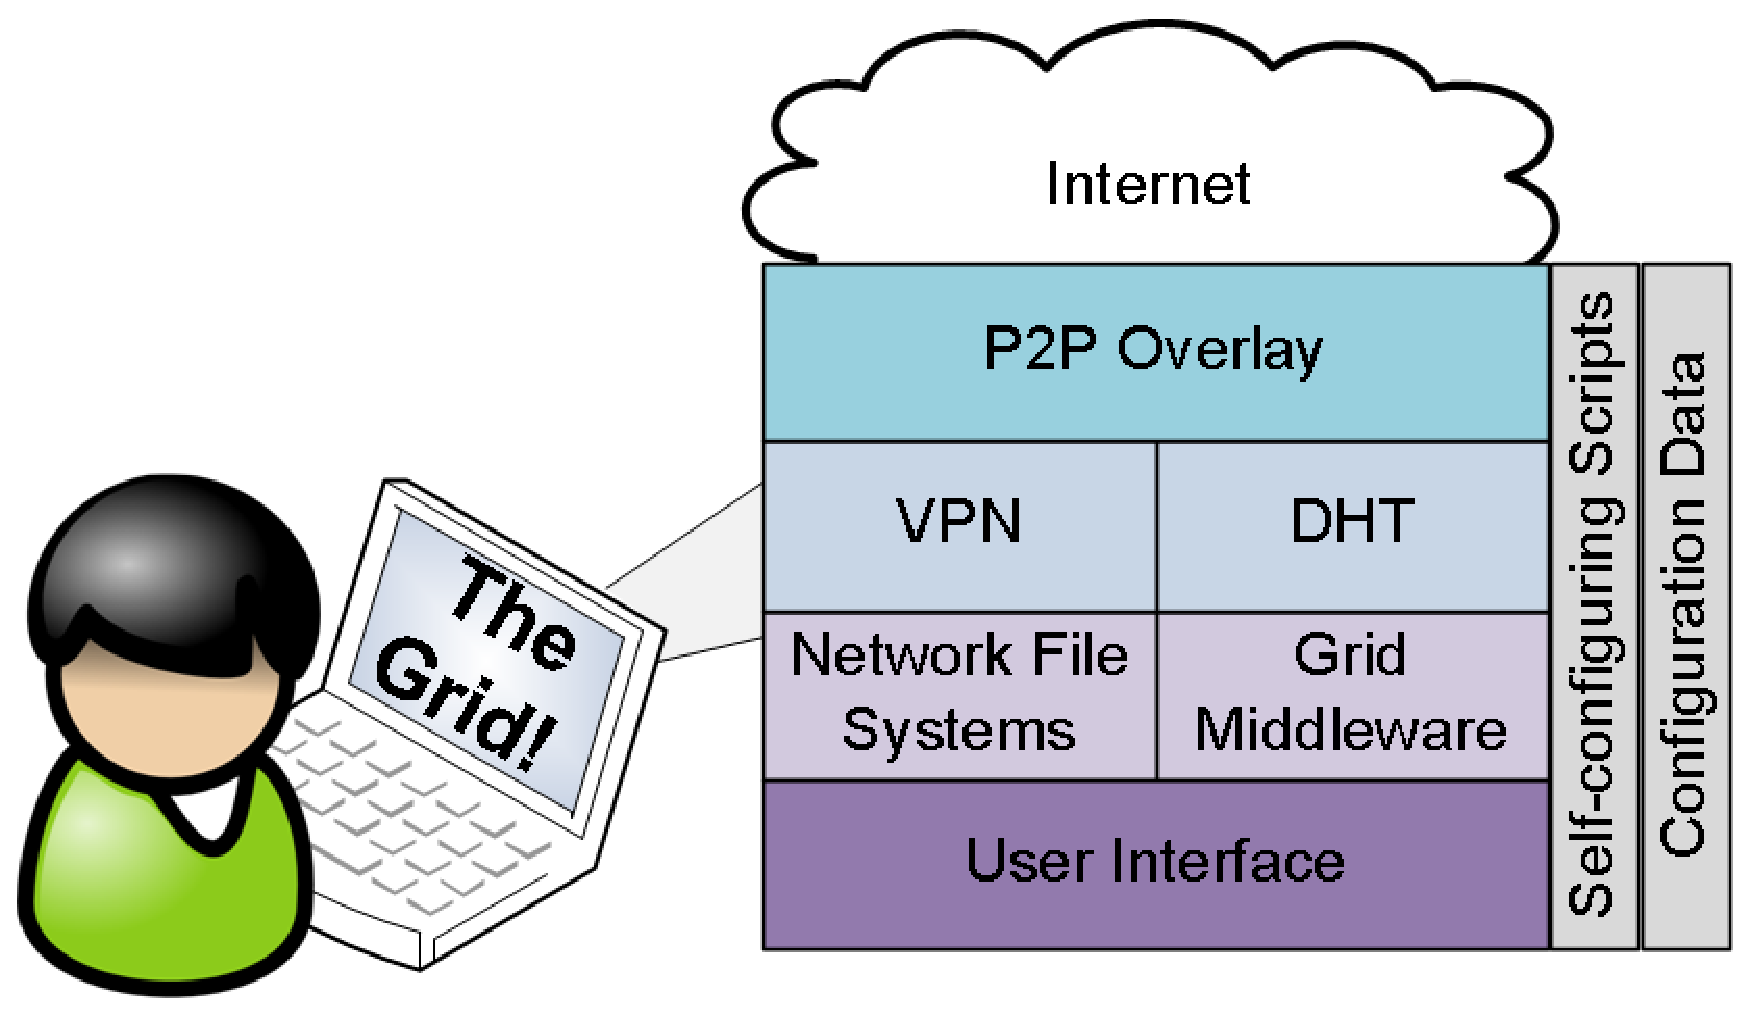
\includegraphics[width=3.75in,angle=-90]{figs/appliance_overlays.eps}
\caption{A ``Grid Appliance'' system consisting of various users and resource
types.  The grid uses the P2P overlay for connectivity through a VPN and
discovery mechanisms through the DHT.  The Grid Appliance software stack
consists of P2P software, VPN, DHT, grid middleware with self-configuring
scripts, and a user interfaces for the middleware.}
\label{fig:appliance}
\end{figure*}

To configure the grid, users and resources interact with a Web interface.  At
this site, users can create or join group-based grids.  Members of the grid are
able to create and download configuration files, which plug into the ``Grid
Appliance'' as a floppy disk or as a file in its file system.  The file
specifies the type and purpose of the ``Grid Appliance'' instance and uniquely
identifies the owner.  Upon first boot, an appliance instance contacts the
``Group Appliances'' site specified in the configuration file to obtain a
certificate authority (CA) signed certificate, after which the system becomes
completely decentralized and connects to other systems through the P2P overlay.  

To justify our techniques, consider the difficulty in combining resources
across disparate networks, which may or may not involve multiple research
groups.  The set up of security, connectivity, and the continuous management of the system may require
an information technology (IT) expert.  Network constraints present another
complexity beyond configuration and organization of distributed resources.
Contributing groups may have resources behind different network address
translators (NATs) and firewalls, preventing direct communication with each
other.  Even assuming that an institution's network administrator is willing to
make exceptions for the grid, additional rules may be required for each new
cluster or resource added internally and externally, quickly becoming
unmanageable.  Our approach embraces decentralized systems behind NATs and
novice grid administrators.

The rest of this paper discusses these challenges in more detail and our
solutions addressing them.  Section~\ref{system} provides an overview of the
``Grid Appliance'' and the systems involved as well as highlights our core
design.  In Section~\ref{middleware}, we present a detailed review of available
grid middleware to address the ambiguity in the previous section.  As described
in Section~\ref{vpns}, the other key component of the system is a P2P VPN that
makes created distributed systems significantly more simple.
Section~\ref{case_study} provides a case study of a grid deployment using
standard grid deployment techniques compared to our ``Grid Appliance,''
describing qualitatively  the benefits of this approach.  Using the system
described in the previous section, Section~\ref{evaluation} presents a
quantitative evaluation of the time taken to self-configure a ``Grid
Appliance'' wide-area virtual clusters.  We share our experiences from this
long running project in Section~\ref{lessons_learned}.  Finally,
Section~\ref{related_work} compares and contrasts other solutions to these
problems.

\section{The ``Grid Appliance'': From a User's Standpoint}
\label{system}

This section highlights the different aspects of the system as shown in
Figure~\ref{fig:system}.  This presents what a first time user would experience
including interaction with the Web site and the services used directly or
indirectly to configure a working grid system.  Later on in
Section~\ref{case_study}, this effort will be compared to the configuration and
use of a manually configured grid.

\subsection{Creating the Grid}

Prior to deploying a grid, users should be aware of the core user components of
the ``Grid Appliance'': understand the group Web site, be able to deploy VMs or
physical resources, and able to use a grid task scheduler (discussed in
Section~\ref{middleware}).  To address users who may not be familiar with these
parts, helpful tutorials are provided on \url{www.grid-appliance.org}.  

\begin{figure*}[ht]
\centering
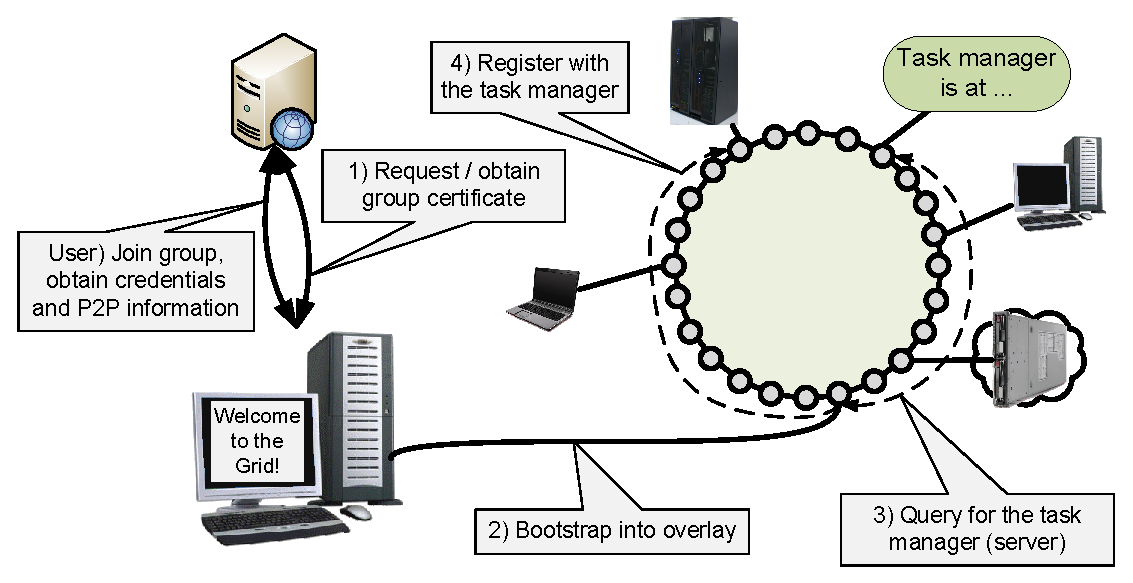
\epsfig{file=figs/system.eps, width=5.75in}
\caption{An example deployment scenario:  obtaining configuration files,
starting the appliance, and connecting with a resource manager.}
\label{fig:system}
\end{figure*}

The process begins with the first step, labeled ``User,'' where a user either
creates a new grid or joins an existing one via groups.  There are two types of
groups: ``GroupVPN'' groups and ``GroupAppliance'' groups. A ``GroupVPN'' group
constitutes a virtual private network that provides connectivity within a grid
and isolation from other grids, while ``GroupAppliance'' groups represent
subsets of a grid.  This approach allows for delegation of responsibilities
across the grid and as a means to ensure higher priority for members of the
same ``GroupAppliance.'' The latter is important in a scenario where multiple
independent departments at a universty or group collaborators across multiple
institutions may desire to share resources together, to take advantage of each
others idle cycles.  Though when a deadline approaches, they will want priority
on their contributed resources.  Without priority, they may avoid a grid
altogether.  Though with the ``Grid Appliance,'' the ``GroupVPN'' allows the
departments to collaborate their resources into a common university grid, while
still maintaining priority to their own resources through ``GroupAppliances.''

Creating a new grid involves the creation of a new a ``GroupVPN'' group
followed by a ``GroupAppliance'' group.  Joining an existing grid requires a
user to join its ``GroupVPN'' group and then a ``GroupAppliance'' group
matching their affiliation or creating their own.  Members of a
``GroupAppliance'' group are presented with the options of obtaining
configuration files to create managers, workers, and clients.  The
configuration data is key to enabling automation of the appliance  The contents
assist the ``Grid Appliance'' scripts in taking an unconfigured appliance to a
configured one through discovery and coordination using the DHT, as described
in Section~\ref{condor}.  The contents of the configuration files are as
follows:

\begin{tabbing}
P2\=P Config:\\
\> List of bootstrap nodes\\
\> P2P security configuration (key, certificate)\\
VPN Config:\\
\> VPN Group name\\
\> Group Web interface URL\\
\> Secret key for obtaining signed certificates\\
\> Group user name\\
Grid Appliance config:\\
\> Appliance type (manager, work, client)\\
\> Administrator ssh key\\
\end{tabbing}

A new grid requires a manager to coordinate workers and clients.  In the
context of traditional cluster and grid middleware, this is the machine that
keeps track of the global task queue and enforces user priorities.  Machines
used only to run tasks are called workers.  Finally, client systems have the
ability to submit tasks and other features useful for interacting with the grid
in addition to the roles of a worker.  While these terms are used loosely in
this discussion, their use is determined by the self-configuring scripts for
the middleware installed.  Section~\ref{condor} presents their relationship
when used with Condor.

Once a user has the configuration files to bootstrap managers, workers, and
clients, they can start ``Grid Appliance'' instances  on physical, virtual, or
cloud machine.  Users can either download a preconfigured VM, start a cloud
instance, or create their own system through the use of package management
systems, like APT and YUM.  To create a new system, users can take an existing
Linux installation, add the ``Grid Appliance'' repository, and install the
packages by executing commands such as ``yum install grid-appliance'' or
``apt-get install grid-appliance.'' Alternatively, this process can be
automated during the installation of the operating system through a preseed or
kickstart file.  The grid configuration files can be added to the system via a
floppy disk for a virtual or physical machine, user data for cloud instances,
or placed in a specific directory inside the system or on a local Web site for
all three types of configurations.  Again, this process can be streamlined with
operating system installation or done afterward.  
 
For users seeking to deploy their own grid rather than join an existing one,
they need to deploy a single manager, and one or more workers and/or clients.
From Figure~\ref{fig:system} step ``1,'' during system boot and without user
interaction, each machine contacts the group Web site to obtain a valid
``GroupVPN'' certificate.  This approach allows a single floppy disk to
bootstrap many systems.  Once the machine has a certificate, it connects to the
P2P overlay whose bootstrap peers are listed inside the configuration file,
``step 2.''  At which point, the machine starts the VPN service running on top
of the P2P overlay, also part of step ``2.'' The self-configuring VPN hides
from the user the complexity of setting up a common fabric that is subject to
network dynamics and connectivity, issues further explored in
Section~\ref{vpns}.  At this point, the machine will automatically obtain a
unique IP Address and find its place inside the grid.  A manager machine will
register itself with the P2P system (not shown), while clients and workers will
attempt to find available managers by querying the P2P overlay, step ``3,'' and
then the managers directly, step ``4.''  The technical details for our approach
with Condor are described in Section~\ref{condor}.

\subsection{Improving User Experience}

With the proceeding steps completed, the grid system has been created.  A user
can submit tasks and receive tasks to run on their systems.  The remaining
issues focus on user access, which needs to address questions including: how do
users easily move files across the grid or into their local machine?  If a user
runs a client in a virtual machine on their desktop, how can the client be
informed to refuse running jobs, while the user is on the desktop?

Systems like these have many potential security issues and its not trivial to
design an approach that balances usability with security.  Our goal is to
secure the system to the point that the only viable attacks are those directly
against the software running on the machine and not poorly chosen passwords or
resources outside of the grid, thus creating a sandbox.  To do so, tasks
running on a remote machine are severly limited in what they are capable of
doing.  File system access is limited to only those files and directories
allowed for everybody and that specific user.  Escalation of privilege attacks
due to poor passwords are prevented by disallowing use of ``su'' or ``sudo.''
Finally, network access is limited to the VPN, thus they are unable to perform
denial of service attacks on the Internet.

For accessibility, users have access to network file systems and remote login.
These services are secured by preventing access to them via the Internet and
the VPN to prevent malicious exploitation.  These servies include a SSH server
and a Samba or Windows File Share with the user name set to that of the name on
the group Web site and the password defaulted to ``password.'' The ``Grid
Appliance'' hosts its own Samba share as oppose to using traditional virtual
machine file shares.  This is the reverse of typical VM approaches, which mount
the hosts file system, but doing so creates potential security risks.  To
access these services, users can add a second Ethernet device, on a trusted
network.  In a virtual machine environment, this may be connected to
"host-only" in other words, only the host machine may use it.  Alternatively in
a cluster, the first Ethernet may be connected to the Internet and the second
to the LAN only.

When running a VM on a desktop, the VM is unable to detect if there is an
active user on the host.  To address these concerns, we have written an agent
that communicates with the client through the second Ethernet device.  The
agent discovers a server through multicast service discovery and verifies that
it is running on the local machine by limiting the discovery to networks other
than that of the default network device on the host.  The agent notifies the
client's server process, whenever a user is accessing the host.  Then the
server will prevent tasks from being scheduled on the local machine until
sufficiently long time has passed since it last heard from the agent, typically
10 minutes.

While grid middleware typically provide data distribution mechanisms, it is important
to also provide support for a common, O/S layer data sharing facility.  For example, an individual worker may only
need a fraction of the data contained within a large file, transferring the
entire file may make use of the grid disadvantageous.  To support these sort of
sparse data transfers, each ``Grid Appliance'' has a local NFS share, which is
exported with read-only permission.  There still exists that challenge that
traditionally in a Unix system a file systems must be manually mounted.
Fortunately, there exist tools to automatically mount file systems, e.g.
autofs. The autofs tools work by intercepting file system calls inside a specific
directory, parsing the directory link, and mounting a remote file system.  In
the ``Grid Appliance,'' this occurs through the path /mnt/ganfs/hostname, where
the hostname is either the IP address or hostname of another instance.
Accessing a file in that path will automatically mount the NFS for that ``Grid
Appliance'' without the need for super-user intervention.  Mounts are
automatically unmounted after a sufficient period of time without any access to
the mounted file system.  

\section{Grid Middleware}
\label{middleware}

Grid middleware is used to connect various distributed resources together in
order to run computing tasks.  These type of systems include resource
management systems like Torque, Condor, and Oracle / Sun Grid Engine (SGE),
which consist of three fundamental components: execute nodes, resource
managers, and submission nodes.  Users access a submission site, craft task
description files, and submit them to a scheduler or resource manager, which
will queue tasks to the various execute nodes to run when available.

\subsection{A Survey of Grid Middleware}

Some of the issues that arise when configuring grids include:  how will users
connect to resources, who will be able to submit jobs, where will the job queue
be located, how can priority be given to local users, how large can the grid
become, and what if any changes will the user need to make to their software to
run it on the grid.  In Table~\ref{tab:grid}, we compare both popular grid
solutions with recent research projects like BonjourGrid~\cite{bonjourgrid} and
PastryGrid~\cite{pastrygrid} that are aimed at resolving some of the more
challenging issues regarding coordination.

\begin{table*}[ht]
\small{
%\setlength{\itemsep}{1pt}
%\setlength{\parskip}{1pt}
\centering
\begin{tabular}[c]{|p{1.4cm}||p{3.475cm}|p{3.475cm}|p{3.475cm}|p{3.475cm}|} \hline
& Description & Scalability & Job queue / submission site & API Requirements \\ \hline \hline
Boinc &
Volunteer computing, applications ship with Boinc and poll head node for data
sets &
Not explicitly mentioned, limited by the ability of the scheduler to handle
the demands of the client &
Each application has a different site, no separation from job queue and
submission site &
Applications are bundled with Boinc and must be written to use the Boinc API
in order to retrieve data sets and submit results to the head node
\\ \hline
BonjourGrid &
Desktop grid, use zeroconf / Bonjour to find available resources in a LAN &
No bounds tested, limits include multicasting overheads and processing power
of job queue node &
Each user has their own job queue / submission site &
None \\ \hline
Condor &
High throughput computing / on demand / desktop / etc / general grid computing &
Over 10,000$^{1}$ &
Global job queue, separate submission site, optionally one per user &
Optional API to support job migration and checkpointing \\ \hline
PastryGrid &
Use structured overlay Pastry to form decentralized grids &
Decentralized, single node limited by its processing power, though
collectivitely limited by the Pastry DHT &
Each connected peer maintains its own job queue and submission site &
None \\ \hline
PBS / Torque~\cite{torque} &
Traditional approach to dedicated grid computing &
up to 20,000 CPUs$^{2}$ &
Global job queue and submission site &
None
\\ \hline
SGE &
Traditional approach to dedicated grid computing &
Tested up to 63,000 cores on almost 4,000 hosts$^{3}$ &
Global job queue and submission site &
None
\\ \hline
XtremWeb &
Desktop grid, similar to Condor but uses pull instead of push, like Boinc &
Not explicitly mentioned, limited by the ability of the scheduler to handle
the demands of clients &
Global job queue, separate submission site, optionally one per user &
No built-in support for shared file systems
\\ \hline
\end{tabular}
\caption{Grid Middleware Comparison}
\label{tab:grid}
}
\end{table*}

Many grids are configured to have a single site for job submission, such that
all users of the system, both local and remote, must have direct access to the
submission site.  At this site, users each have a unique account for their use
and have the ability to execute programs and store files.  This means that an
administrator must explicitly create an account and that the user must be
trusted.  A malicious user could run an application that escalates privileges,
distribute copyrighted materials, or interfere with others use of the grid.
The goal of the ``Grid Appliance'' is to isolate users and make them
self-sufficient, in doing so, we require that submission sites be created on
demand and potentially be single user and optionally multiuser.  By doing so,
users are never given explicit accounts on privileged resources inside of
secure environments.  Instead all job submissions occur from their own
resources.

Having a single job queue can lead to unfair sharing of resources, for example,
consider a multi-site grid with a single job queue.  If the managers of the job
queue were in dire need for resources, they could manipulate the system in
order to obtain higher priority on all resources, abusing their power and
obtaining an unfair portion of all grid resources.  On the other hand, a user
or a site that provides resources for the grid should have high priority on
their own resources, otherwise, their motivation for sharing would be limited,
because they could just as well remove their resources from being shared
whenever the user or a member of the site wanted to use them.  Having to deal
with these issues is undesirable and could inevitably lead to a fractured grid,
as many users may simply desire for a simpler setup, where there is no concern
about ensuring privilege on their own resources.  Furthermore, when grids are
financed by third parties, the third parties like to receive statistics about
their use, if a member of a grid were to remove their resources every time a
local user needed them, those results would not be recorded nor available to
the third party.  We believe at a minimum each site should have the opportunity
to run their own job queue, at a minimum their will be a job queue for the
entire network, and optionally, each submission site will behave as a job queue
in a completely decentralized system.

While its not particularly common, some systems, like Boinc, require that a
user wishing to deploy tasks on a grid compile their software using particular
APIs.  Some, like Condor, provide optional APIs to provide extended features
like process check-pointing and migration.  Having firm requirements that force
users to write specialized code may work for certain environments, but doing so
increases the entry barrier and may provide too much challenge for courses in
grid computing.  Having optional requirements, lets dedicated users take
advantage of special features without affecting the use of less complex tasks.

\addtocounter{footnote}{1}
\footnotetext[\value{footnote}]{\url{http://www.cs.wisc.edu/condor/CondorWeek2009/condor\_presentations/sfiligoi-Condor\_WAN\_scalability.pdf}}
\addtocounter{footnote}{1}
\footnotetext[\value{footnote}]{\url{http://www.clusterresources.com/docs/211}}
\addtocounter{footnote}{1}
\footnotetext[\value{footnote}]{\url{http://www.sun.com/offers/docs/Extreme\_Scalability\_SGE.pdf}}

Considering these three issues:  submission site, job queue site, and API
requirements, we firmly believe that out of the potential choices Condor
matches best.  While systems like PastryGrid and BonjourGrid are developing
nicely, our attempts to get PastryGrid online failed as Pastry suffers from
dynamic bootstrapping issues and PastryGrid was unable to actually execute our
submitted tasks and both do not support priority nor fairness.  Also, systems
like PBS/Torque and SGE are significantly centralized and while using systems
that allow cross-domain grids through middleware like Globus~\cite{globus}
could potentially enable these systems to meet our goals, we found the end
result too complex.  Boinc is completely inappropriate for our approach as it
really works well when used to facilitate a single project from a central
point.

\subsection{Configuring Grid Middleware through the DHT}
\label{condor}

To efficiently and transparently construct wide area grids, we employ a DHT.
To do so, a manager places its IP address into the DHT at the key
\emph{managers}.  When workers and clients join the grid, the systems
automatically query this key and configure to report to one or more managers,
application dependent.  Likewise, managers can query this key to learn of other
managers to coordinate with each other.

Of the resource management middlewares that we have surveyed, Condor matched
closest with our goals due to its decentralized properties and focus on desktop
grids and voluntary computing.  As described above, most of the available
cluster and grid software do not easily support multiple submit points, in
fact, most require another piece of software to bridge the gap between cluster
and grid, or more explicitly distribution of the system.

\begin{figure*}[h!t!]
\centering
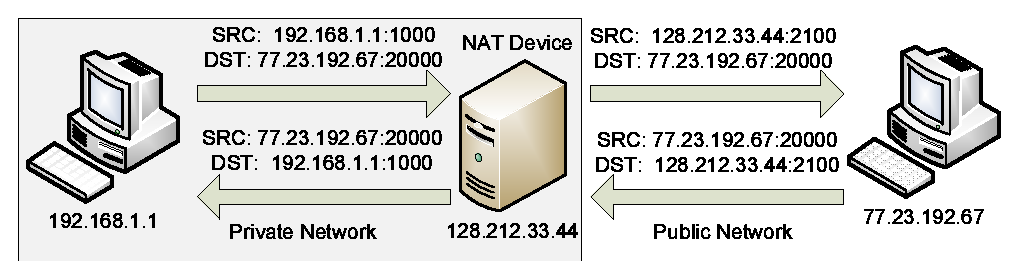
\epsfig{file=figs/NAT.eps, width=5in}
\caption{A typical NAT interaction. The peer behind a NAT has a private address.
When the packet is sent through the NAT, the NAT translates the source information
into a public mapping, keeping the original source information so that if a
packet from the remote peer comes back, it can be translated and delivered to
the original source.}
\label{fig:nat}
\end{figure*}

Further motivating Condor is the ease in adding new resources.  To add new
resources to a Condor system, an execute or submission node must have the IP
address for the manager, the rest of the system organization is performed
entirely transparent to the user.  Conversely, in SGE and Torque, after
resources have been added into the system, the user must manually configure the
manager to control them.

Finally, Condor supports opportunistic cycles.  Most scheduling software
assumes that resources are dedicated and do not handle cases, where other
processors or a user also interact with the system.  Condor, however, can
detect the presence of other processes or a user and suspend, migrate, or
terminate a job.

A caveat to our approach is the requirement of a manager, while the system
organizes through a decentralized means, it still results in a distributed
system relying heavily on a small subset of nodes.  For future work, we are
investigating means to completely decentralized the manager node, potentially
by making each node a manager for its own node and through decentralized
resource discovery and priority ranking algorithms.  In the meantime, we have
taken advantage of a feature known as ``flocking'' in Condor.  Flocking allows
submission sites to connect to multiple managers.  This serves two purposes: 1)
to provide transparent reliability by supporting multiple managers and 2) users
can share their resources through their own manager.  

To configure Condor, we store managers IP addresses into the DHT using the key
\emph{managers}.  When a new peer joins, it queries the DHT, obtains the list
of all managers, and randomly selects one as its primary manager.  The rest are
set to flocking.  If the system prefers managers from its group, it will
randomly contact each manager in an attempt to find a match, selecting one at
random if no match is found.  If no managers are found, the process repeats
every 60 seconds.  Once a manager has been found, it is checked every 10
minutes to ensure it is online and additional managers that have come online
are added to the flock list.

\section{The Motivation for VPNs}
\label{vpns}

As of 2010, a majority of the Internet is connected via Internet Protocol (IP)
version 4, which is quickly approaching its limit of available addresses,
$2^{32}$ (approximately 4 billion).  With the Earth's population at over 6.8
billion and each individual potentially having multiple devices with Internet
connectivity, the IPv4 limitation is becoming more and more apparent.  There
are two approaches to addressing this issue:  1) the use of NATs to enable many
machines and devices to share a single IP address but preventing bidirectional
connection initiation, and 2) IPv6 which supports $2^{128}$ addresses.  The use
of NATs, as shown in Figure~\ref{fig:nat}, complicates grid systems that
require all-to-all communication, which include all of those which we consider.
In addition, firewalls may prevent peers from receiving incoming connections.
And while the eventual widespread use IPv6 may eliminate the need for address
translation, it does not deal with the issue of firewalls, and the future of
NATs in IPv6 is unclear.

The use of VPNs motivates beyond the impetus for traversing NATs and firewalls.
With a VPN, users can avoid the headaches associated with dynamic IP addresses,
as each VPN instance can claim and maintain a globally unique IP address and,
regardless of the machines physical location and mobility, ideal condition for
laptop users.  In addition, it abstracts the user from having to be concerned
about network addresses.  For example, when using machines across networks or
even a virtual machines inside the same LAN but behind virtual machine manager
NATs, users must be wary of all nodes in the systems ability to connect with
each other.  When using a VPN, these considerations are unwarranted, the grid
software need only concern itself of the VPN and the direct connectivity
provided through it.

Our work relies on a group enabled IPOP VPN called GroupVPN~\cite{groupvpn}.
IPOP through its underlying P2P infrastructure supports NAT traversal allowing
peers behind NATs and firewalls to communicate directly and indirectly through
relays in the P2P system.  The VPN enables many of the key features in the
``Grid Appliance.'' For example, if there were not a VPN, users of MPI and
Hadoop would need to ensure that all resources were bridged to the LAN and not
through a VM NAT, the typical configuration, otherwise the multicast message
would not be delivered to all participants.  The VPN software supports the
ability to self-organize using existing infrastructures including IP multicast,
public overlays, and Xmpp as described in our previous
work~\cite{bootstrapping}.  This is in contrast to other VPNs like
Hamachi~\cite{hamachi}, OpenVPN~\cite{openvpn}, Tinc~\cite{tinc},
Violin~\cite{violin}, ViNe~\cite{vine}, or VNET~\cite{vnet}, that are either
centralized and require a dedicated node to coordinate peers or decentralized
solutions that require manual configuration of links between peers.

Using the aforementioned techniques ``Grid Appliances'' can be constructed in
one of two ways: local and wide area.  The ``Grid Appliance'' ships with two
default configurations, one that connects users to a globally available public
system and another that allows for LAN only grids.  Local grids can be
constructed by booting the appliances, which will then use multicast
self-discovery to find other resources, create the DHT overlay, and then form
VPN links.  Alternatively, the user can connect to the default publc system or
use ``GroupAppliances'' to create and manage their own grid, both of which
bootstrap from a public shared DHT overlay.  This does not prohibit more
advanced users from downloading our ``GroupAppliances,'' as its available as a
VM, and host their own DHT overlay.

\section{A Case Study on Deploying a Campus Grid}
\label{case_study}

We now present a case study to explore the qualitative differences in deploying
a campus grid using traditional techniques versus a grid constructed by ``Grid
Appliance.''  One of the target environments for the ``Grid Appliance'' is
resources provided in distributed computer labs and many small distributed
clusters on one or more university campus as shown in
Figure~\ref{fig:unconnected}.  In this case study, we examine approaches to
setting up a grid connecting these different sets of resources using commodity
components in contrast to the ``Grid Appliance.''

\begin{figure}[ht]
\centering
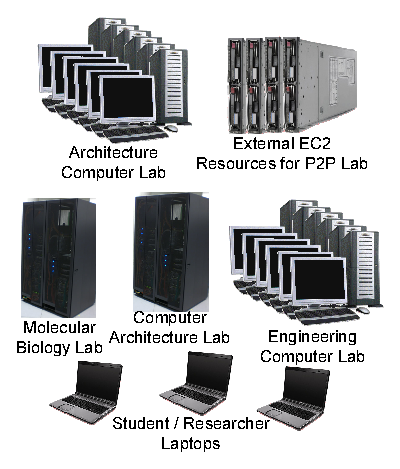
\epsfig{file=figs/unconnected.eps, width=2.75in}
\caption{A collection of various computing resources at a typical university.}
\label{fig:unconnected}
\end{figure}

\subsection{Traditional Configuration of a Campus Grid}

The first step in joining the resources is determining the network
configuration of the system.  Condor like most other push based schedulers
requires that the submission sites have direct continuous network access to the
workers in the system.  To deal with potential network asymmetries, all systems
can be placed on a common VLAN, though this may be complicated across a campus
and even more difficult if resources were to include other universities or
cloud resources.  Thus to deal with these potential network asymmetries, the
user would need to deploy a VPN.  The most straight-forward approach would be
to deploy an OpenVPN on the manager node.  Using OpenVPN, like most VPNs,
requires that each node be pre-configured with a unique key and
signed-certificate, a tedious process that takes time and effort.  The problem
with using most VPNs is there lack of support for dynamics in the system.  If a
node in the critical path between two nodes goes offline, network communication
will be broken.  The only VPN resilient to these types of failures is IPOP as
there are no critical nodes between two communicating peers.

With the grid in place, users will want to submit jobs.  A global submission
site will allow for a simpler though not necessarily trivial network
configuration.  Whereas having each user supply their own submission site would
require nearly all-to-all connectivity in the system, which is not very common
on a university campus.  So while a global submission site may reduce
networking configuration costs, it increases administration costs both in terms
of utilities and personel.  A global submission site requires administration,
Boinc makes claims that a fully functional system should require approximately
20 hours a week of effort to maintain this system.  Using a global submission
site will also cost computing and electrical resources, as more users are added
to the system, file system space, memory, and processing power may be needed on
the submission site.  Alternatively, if each user supplies their own submission
site, all these issues will be negated though all the users will need to
maintain uninterupted connectivity to the worker machines.  Regardless of the
path taken, someone will have to sign a new certificate for each resource a
user wants to connect to the resource or create a new account for each new
user.

Once those details have been fleshed out, the next consideration is ensuring
homogeneity on the resources.  If there are different system configurations on
the various machines, an application that works well on one platform could
cause a segmentation fault on another, through no fault of the developer, but
rather due to library incompatibilities.  The easiest way to deal with this
approach is to use a virtual machine and there are many groups that do this.
Owners of the clusters could either use these virtual machines or manually
install the same software on their machines.

Once the machines are fully installed, they will need to be configured to point
to the global job queue or server, which in Condor can be multiple individual
queues as well as be separate from individual submission sites.  Condor
supports a high availability mode as well as having parallel queues via
flocking.  Regardless of which approach is taken, the IP address or hostname of
these end points will need to be added to each of the resources.  If they ever
change, each machine will need to be reconfigured to point to the new
locations.

The final component deals with fairness, which has to aspects:  users who
contribute resources should have priority on them and if a user is directly
accessing a computer lab's resource directly it should not be hampered by
remote users' jobs.  To support user and group based priorities, Condor has
mechanisms that can be enforced at the server that allows for abitrary means to
allow one user to have higher priority than another user on a specific machine.
This is done through specifying on the worker machine two variables, the
contributing users name and/or the contributing groups name.  When the server
receives a job request, it compares the submission nodes user name / group name
with that of workers, if there is a mapping that user will get priority over
other users.  This can either be realized by the next time the resource is
available, it will be given to that user or by pre-empting a non-owners job
from that resource.

\begin{tabbing}
Th\=e \=format for this configuration is as follows:\\
\> Job queue (server):\\
\> \> NEGOTIATOR\_PRE\_JOB\_RANK = 10 * (MY.RANK) \\
\> Worker:\\
\> \> GROUP\_RANK = TARGET.Group =?= MY.Group \\
\> \> USER\_RANK = TARGET.User =?= My.User \\
\> \> RANK = GROUP\_RANK $\vert\vert$ USER\_RANK \\
\>  Worker and Submitter:\\
\> \> Group = "Group's Name"\\
\> \> User = "User's Name"
\end{tabbing}

The huge caveat is that even with this in place, if there is no mechanism for
verifying the identity of the submitting node, a malicious user can obtain
priorities not granted to them.  In the Grid Appliance, this is addressed by
storing this information inside the certificate of the VPN, which the server
can request using a XMLRPC link to the P2P VPN.  In other systems, this may
require accessing a centralized user database or requiring all users in Condor
to use a certificate.

A campus computing lab will lose its purpose if those directly using lab
resources do not have priority over remote users.  If the Condor is running
natively on the host, the administrator can enable Condor features that monitor
for keyboard and mouse movement that will bump jobs off the machine.  Though
most likely, in most common cases virtual machines will be running on the
desktops.  If this is the case, there is not a very intuitive solution on
informing Condor running on the virtual machine, that a user is actually on the
host.  For the Grid Appliance, our solution was to run an agent that monitors
usage on the host and reports it to the virtual machine.  Discovering the
existence of a virtual machine only requires that the VM have a host-only
interface.  The agent will send multicast discovery messages to all the VM
interfaces on the host and if it discovers a VM will then send notifications of
usage to a service on VM.  That service will in turn simulate an active user
inside the VM, causing jobs on the VM to be suspended, migrated, or removed.

Further motivating the desire for having multiple submission sites is desire
for users to the ability to access their data files through NFS.  While it may
be easier to have a single NFS mount on all the workers, it will also add
additional costs to the global submission node.  Earlier we described how we
use autofs to automatically mount NFS stores from submission nodes.  This same
approach could be used in the case of a manually configured grid.  It would
require that each machine was configured the same way though.

\subsection{Grid Appliance Configuration of a Campus Grid}

All these considerations are exactly the reasons why ``Grid Appliance'' and its
associated group Web interface are desirable for small and medium scale grids.
The first component is deciding which Web interface to use, the public one at
\url{www.grid-appliance.org} or another one hosted on their own resources,
similarly the users can deploy their own P2P overlay or use our shared overlay.
At which point, users can create their own VPN groups for different grids and
then their grid groups to ensure priority on their own resources.

The Web site enforces unique names for both the users and the groups.  Once the
user has membership in a ``GroupAppliance'' group, they can download a file
that can be used automatically configure their resource.  This means obtaining
a signed certificate, configuring the group information in Condor, connecting
to a decentralized VPN, and discovering the server in the grid.  The user does
not need to be concerned about location thanks to the VPN or changes in the
configuration of the grid thanks to decentralized discovery of the server.
Finally, the ``Grid Appliance'' approach ensures homogeneity as all users
install the same packages on the same platforms.  Whereas a traditional grid
would require users to conform with each other or deal with the
incompatibilities across machines.

\subsection{Comparing the User Experience}

After a user has obtained an account and done all the other appropriate steps
to connect with the grid, in the traditional setup, they will SSH into the
submission site.  Their connectivity to the system is instantaneous, their jobs
will begin executing as soon as it is their turn in the queue, which can be
instanteous in a lowly utilized system.

The procedure taken by the ``Grid Appliance'' is slightly different.  When the
user first boots a ``Grid Appliance,'' sometimes it will have already connected
with the server prior to the user having access to a command prompt and
sometimes not.  Typically a ``Grid Appliance'' will be completely ready within
30 seconds or less, though our current approach relies on polling the state of
the P2P overlay and the VPN rather than using events, which may further lower
this time.  To ensure users that everything is progressing normally, we have a
window appear telling them the state of the system, including the state of the
VPN and Condor.

Once a user has access to a prompt, they can submit jobs.  Their jobs will too
begin executing as soon as it is their turn in the queue; however, before a job
can be executed a direct VPN link must be established between the submission
site and the task worker.  The amount of time required varies on the network
configuration, though in all cases a direct link will be established.
Sometimes that direct link consist of routing through a well chosen proxy as
discussed in~\cite{groupvpn}.

With the ``Grid Appliance,'' users are not limited to accessing their files
through SSH and SFTP.  We have also configured the ``Grid Appliance'' to
support a local Samba mount or Windows file share.  Something recognized as not
being safe to do on an open / untrusted network but is safe to do since the
``Grid Appliance'' runs on the users local resources.

\section{Evaluation}
\label{evaluation}

In the previous section, we qualified why the approach was easier than
configuring a grid by hand, though by doing so we introduce overheads related
to configuration and organization.  This section verifies that these overheads
do not conflict with the utility of our approach.  The tasks in this evaluation
are to determine the time required to start a grid individually at multiple
sites individually and then cumulatively.  We compare a statically configured
grid versus our dynamic ``Grid Appliance.''  The three environments chosen are
Amazon's EC2 supporting a simple 1:1 NAT, University of Florida directly behind
an ``iptables'' NAT and then a Cisco NAT, and finally a Future Grid at
University of Indiana's using Eucalyptus behind what appeared to be an
``iptables'' NAT.

Prior to beginning the evaluation a manager and submission node are started and
connectivity between the two are verified.  In the case of the static system,
OpenVPN is run from the manager node, which has been assigned a static IP
address.  We ran through the experiments enough to ensure that we were
measuring system delays due to configuration of the grids and not the
underlying systems, i.e., the unpredictable behavior of the underlying systems.
We measured the time from when the last grid resource was started to the time
it reported to the manager node, Figure~\ref{fig:connect} as well as the time
required for the submit node to queue and run a 5 minute job on all the
connected workers, Figure~\ref{fig:run}.  The tests were run on 50 resources in
each environment and then on a grid consisting of all 150 resources with 50 at
each site.

\begin{figure}[ht]
\centering
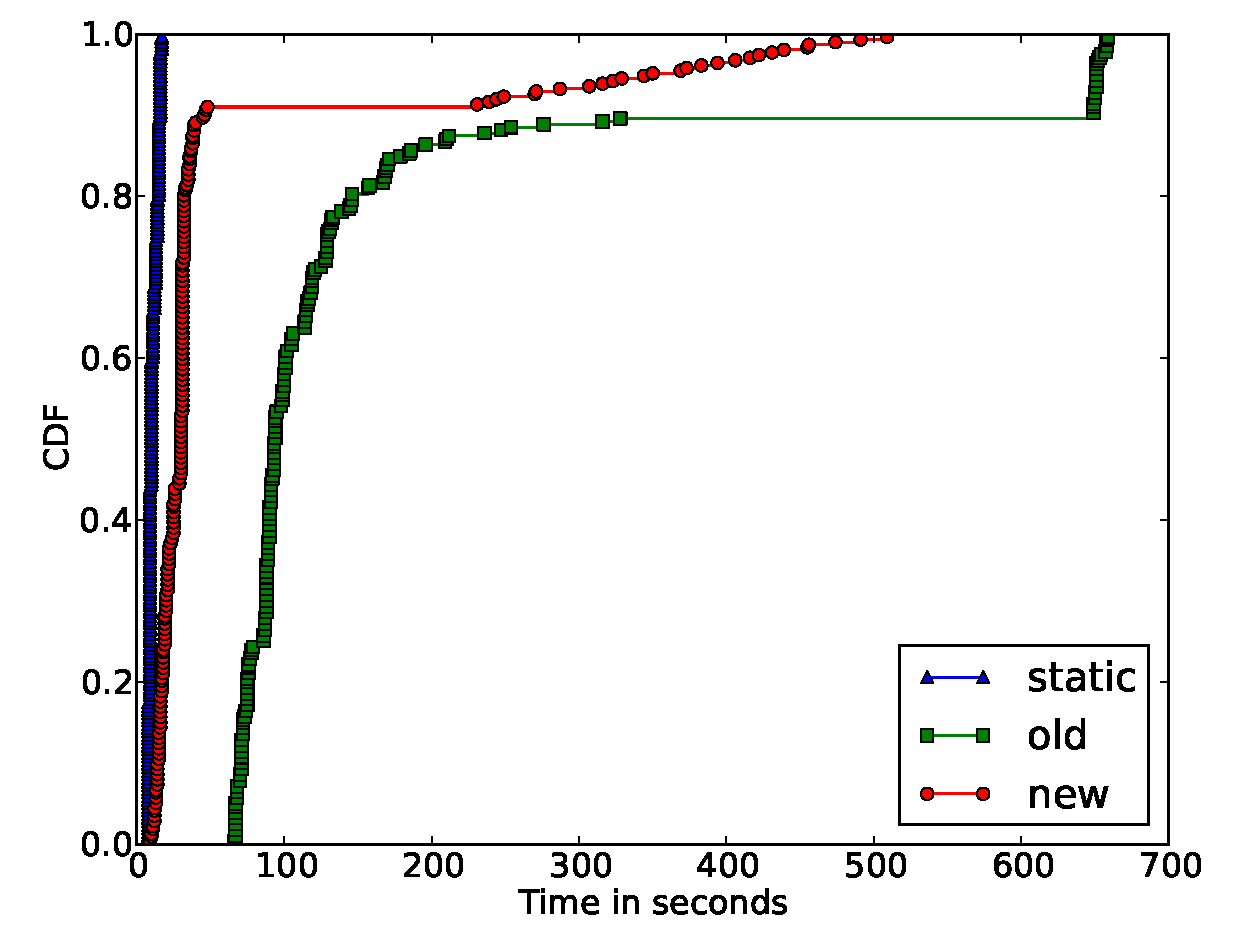
\epsfig{file=figs/connect.eps, width=2.75in}
\caption{Comparison of times to construct a grid in various environments using
both a statically configured grid and a grid constructed by the ``Grid Appliance.''}
\label{fig:connect}
\end{figure}

\begin{figure}[ht]
\centering
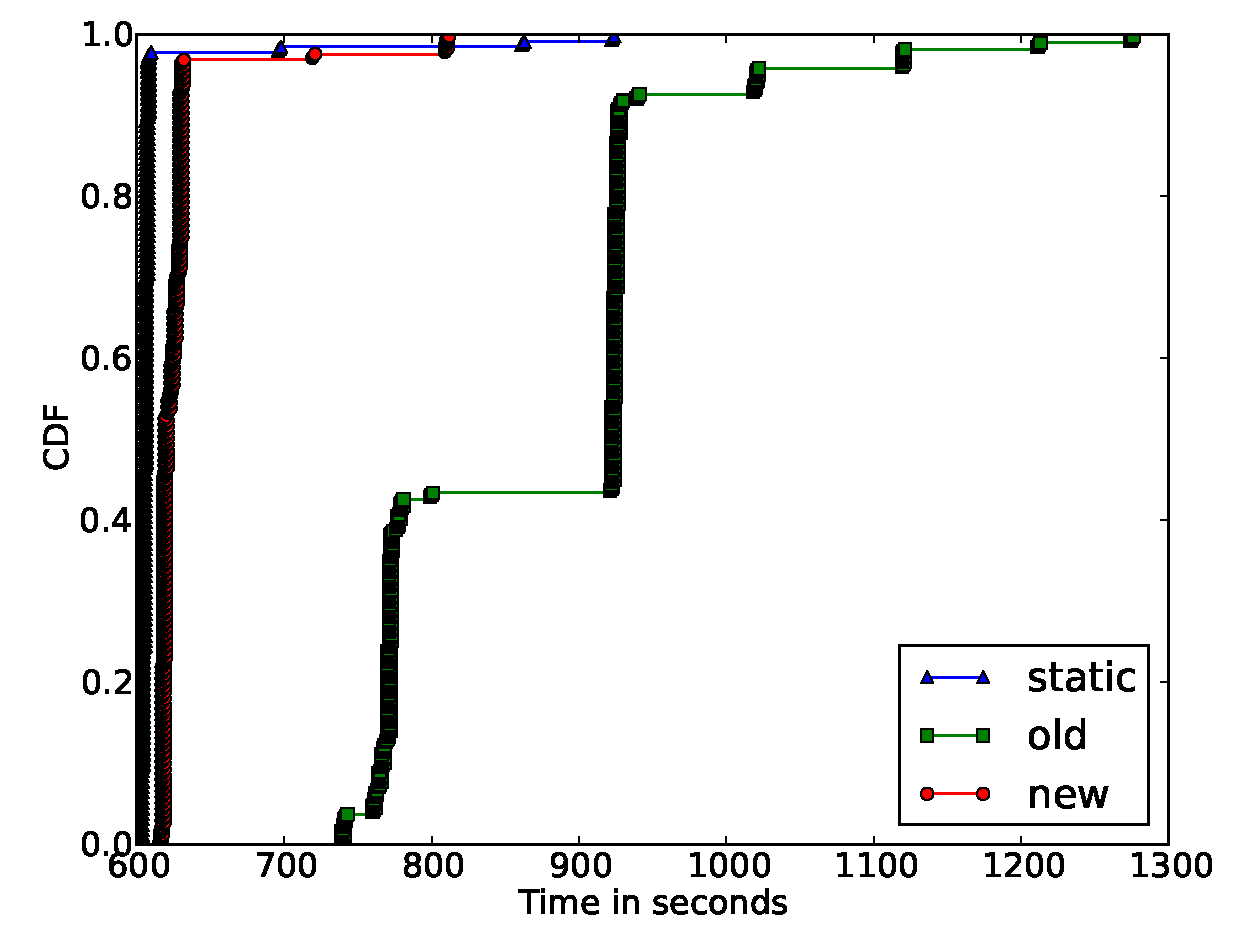
\epsfig{file=figs/run.eps, width=2.75in}
\caption{Comparison of times to run a 300 second job in various grids configured
statically and through the ``Grid Appliance.''}
\label{fig:run}
\end{figure}

The results make it very clear that the overheads introduced through a
decentralized, P2P VPN are minimal and that the time to connected is not
significantly longer than a statically configured environment with a
centralized VPN.  The current ``Grid Appliance'' relies on polling and uses
very lose timing, so as to not hammer the system.  Either shrinking those times
or moving to an event based system should significantly improve the speed at
which connectivity occurs.  

\section{Lessons Learned}
\label{lessons_learned}

In this section, we will present some of our previous experiences in using and
developing the Grid Appliance that were not obvious when we started.  A
significant component of our experience stems from the computational grid
provided by Archer~\cite{archer}, an active grid deployed for computer
architecture research, which has been online for over 3 years.  Archer
currently spans four seed universities contributing over 500 CPUs as well as
contributions and activities from external users.  The Archer grid has been
accessed by over hundreds of students and researchers submitting jobs totaling
over 400,000 hours of job execution in the past two years alone.

The Grid Appliance has also been utilized by groups at the Universities of
Florida, Clemson, Arkansas, and Northwestern Switzerland as a tool for teaching
grid computing.  While Clemson and Purdue are constructing campus grids using
the underlying VPN, GroupVPN / IPOP, to connect resources together.  Recently,
several private small-scale systems have come online using our shared system
available at \url{www.grid-appliance.org} with other groups constructing their
own independent systems.  Feedback from users through surveys have shown that
non-expert users are able to connect to our public Grid appliance pool in a
matter of minutes by simply downloading and booting a plug-and-play VM image
that is portable across VMware, VirtualBox, and KVM.

\subsection{Stacked File Systems}

Configuring systems can be difficult, which makes it important to have the
ability to share the resulting system with others.  The approach of actually
creating packages can be overly complicated for novices, to adress this
concern, our original ``Grid Appliance'' supported a built-in mechanism to
create packages through a stackable file system using copy-on-write, as
describe in~\cite{vtdc}.  The appliance at that time ran only on VM consisting
of 3 disks: the ``Grid Appliance'' base image, the software stack configured by
us; a module; and a home disk.  In normal usage, both the base and module
images are treated as read-only file systems with all user changes to the
system being recorded by the home image, as depicted in
Figure~\ref{fig:stackfs}.

\begin{figure}[ht]
\centering
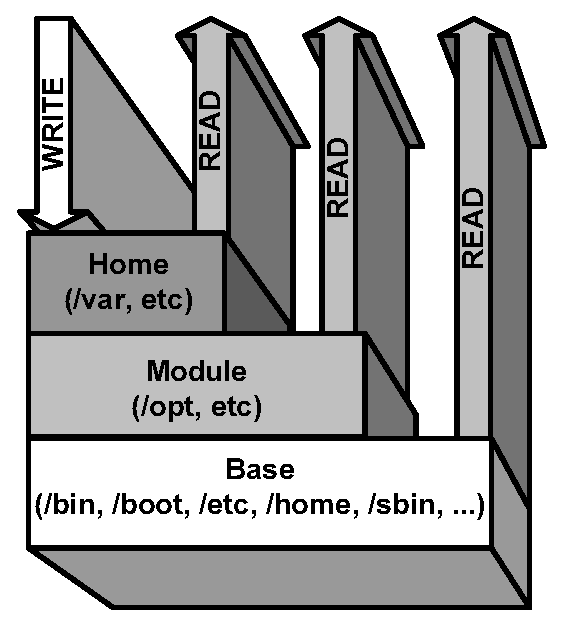
\epsfig{file=figs/stackfs.eps, width=1.75in}
\caption{Example of a stackable file system from our previous ``Grid
Appliance.''  A file will be read from the top most file system in the stack
and all writes are directed to Home.}
\label{fig:stackfs}
\end{figure}

Users could easily upgrade to new versions of the ``Grid Appliance'' by
replacing their base image with a new one, while keeping their module and home
disks.  While the purpose of the module was to allow users to extend the
configuration of the ``Grid Appliance.''  To do so, the user would launch into
developer mode, where all changes would be written to the module image,
rendering the home image unused.  Upon completing the changes, a user would run
a script that would clean the system and prepare it for sharing.  A user could
then share the resulting module image with others.

While there were users for this approach, the issues with it made it
unattractive to continue using.  First, there exists no kernel level support
for stackable file systems, we had to add UnionFS~\cite{unionfs} to the kernel,
adding the weight of maintaining a kernel unto our shoulders.  While there does
exist FUSE, or filesystem in userspace, solutions, using those properly require
modifications to the initial ramdisk, reproduced automatically during the
installation of every new kernel, furthermore, our experience with them
suggests they are not well suited for production systems.

The approach was also limited to VMs, hosts such as clouds and physical
resources could not, easily, take advantage of it.  So while we still think the
concept is great, we have removed it from our mainline appliance.  We feel that
the future work for this type of application will be to allow users to
configure a system and then make it easy for them to create packages.  Doing so
will allow the packages to be significantly more portable and less
configuration headaches.  Also, to deal with upgrades, we use standard package
management, so users do not need to deal with VM disk images to upgrade.

\subsection{Timing in Virtual Machines}

% Maybe remove 

Certain applications, particularly license servers, are sensitive to time.
When constructing a grid consisting of many distributed resources, there is a
good possibility that time will be wrong somewhere.  With regards to VMs,
VMWare~\cite{vmware_timing} suggests synchronizing with the hosts time and to
avoid using services like NTP (network time protocol), which may have adverse
affects on timing inside the virtual machine.  Our experiences recommend the
opposite, we have experienced drastic timing jumps and significantly off
virtual clocks due to host clocks being set incorrectly.  It seems the virtual
clock would force an immediate jump in timing for the virtual clock, which
could be quite significant if the VM had not been scheduled recently enough.
NTP, on the other hand, gradually corrects time.  This major jump would cause
the system to completely stall due to software that was unable to handle the
unreliability in time.  Because in many cases, the VMs run on machines that are
not owned by the VM owner, correcting the host time is not possible.  Our
conclusion is that developers should be wary when using virtual timing,
especially if they are constructing distributed systems.  Rather they should
consider using NTP, especially if your application will run on a device where
the user may not have the ability to change the hosts timing.  It should be
noted that the paper from VMWare does not explicitly recommend against NTP,
just that it can be difficult to properly to configure.  For example, if a
solitary NTP server is chosen, it may be offline or behave erratically, an
issue typically bypassed when using the default NTP server provided the
operating system distributor.

\subsection{Selecting a VPN IP Address Range}

The challenging to deploying a VPN is ensuring that the address space does not
overlap with that over the environments where it will be used.  If there is
overlap, users will be unable to connect to the VPN.  Doing so will confuse the
network stack, because there would be two network interfaces connected to the
same address space but not the same network.  One potential solution is for a
user to run the VPN behind a NAT, like inside a VM behind a VM NAT or a
cluster beind a NAT device.

Users of the ``Grid Appliance'' should not have to concern themselves of these
issues.  Prior work on the topic by Ala Rezmerita et al.~\cite{pvc} recommended
using the experimental address class E ranging between 240.0.0.0 -
255.255.255.254, though this requires Linux kernel modifications.  Though with
the amount of bugs and security fixes regularly pushed into the kernel,
maintaining a forked kernel requires a significant amount of time, duplicating
the work already being performed by the OS distribution maintainers.  This also
limited deployment in physical and cloud machines.  Users that wanted to
multipurpose a physical resource may not want to run a modified kernel, while
in most cloud setups the kernel choice is limited.

We have since moved towards using the 5.0.0.0 - 5.255.255.255 address range.
Like the class E address space it is unallocated, but it requires no changes to
any operating systems.  The only limitation is that some other VPNs also use
it, thus a user would not be able to run two VPNs on the same address space
concurrently.  This approach is much better than providing kernels or dealing
with network address overlaps.  Interestingly, even with this in place, we
still see some ``GroupVPNs''  using address ranges in normal private network
address ranges for the VPN, like 10.0.0.0 - 10.255.255.255 and 192.168.0.0 -
192.168.255.255.

\subsection{Securing the VPN and Overlay}

Our original design secured the virtual network through a kernel level IPsec
stack.  A model kept through our first generation Archer deployment and
GroupVPN.  The problem with this approach is that securing links of the VPN
only partially secures the P2P VPN and using IPsec, which is not trivially
configured, to pre-configured environments.  Securing the P2P layer is
important, otherwise malicious users could easily derail the entire system, but
securing with IPsec would practically negate the benefits of the P2P system,
because of network configuration issues related to NATs and firewalls.

To address these, we implemented a security system directly into the P2P
system, thus securing both VPN and P2P communication.  The security filter
supports both DTLS and a protocol similar to IPSec.  The overheads of using
security turned out to be significantly small, as we explored
in~\cite{bootstrapping}.

\subsection{Towards Unvirtualized Environments}

Users comfortable with the system and wanting to dedicate computers to their
``Grid Appliance'' grid wanted to remove the overheads of using a VM as well as
being able extend their compute resources into the cloud.  So while, we could
create shareable cloud instances, but a physical machine is a little more
complicated as it requires specialized non-standard software to create a
shareable image.  Especially since other machines may have different hardware
configurations that may actually prevent reusing a shared image.

Due to requests from users wanting better integration with physical machines
and as a result of moving away from stackable file, we move towards creating
installable packages.  Also, we improved the VPN to support a router mode,
whereby a single VPN can be used by many machines inside a LAN.  The
implications of packages mean that users can easily produce ``Grid Appliances''
from installed systems or during system installation.  While the VPN router
allows resources inside a LAN to communicate directly with each other rather
than through the VPN.  That means if they are on a gigabit network, they can
full network speeds as opposed to being limited to 20\% of that due to the VPN,
this was discussed more in our previous work~\cite{sc09}.

\subsection{Advantages and Challenges of the Cloud}

We have had the experience of deploying the ``Grid Appliance'' on three
different cloud stacks:  Amazon's EC2~\cite{ec2}, Future Grid's
Eucalyptus~\cite{eucalyptus}, and Future Grid's Nimbus~\cite{nimbus}.  All of
the systems, encountered so far, allow for data to be uploaded with each cloud
instance started.  The instance can then download the data from a static URL
only accessible from within the instance, for example, EC2 user data is
accessible at \url{http://169.254.169.254/latest/user-data}. A ``Grid
Appliance'' cloud instances can be configured via user-data, which is the the
same configuration data used as the virtual and physical machines, albeit zip
compressed.  The ``Grid Appliance'' seeks the configuration data by first
checking for a physical floppy disk, then in specific directory
(\url{/opt/grid\_appliance/var/floppy.img}), followed by the EC2 / Eucalyptus
URL, and finally the Nimbus URL.  Upon finding a floppy and mounting it, the
system continues on with configuration.

Beyond the use of extending into clouds for on-demand resources, they are also
very convenient for debugging.  Doing so on Amazon though is not free.
Fortunately, grid researchers now can have free access to Future Grid with both
Eucalyptus and Nimbus style clouds.  We did have to do some tinkering to get
these systems to work.  First, because the user data is binary data and the
communication exchange uses RPC, which may have difficulty handling binary
data, it must be converted to base64 before transferring and converted back
into binary data afterward.  EC2 handles this transparently, if using
command-line tools.  Unfortunately, Eucalyptus and Nimbus do not, even though
Eucalyptus is supposed to be compatible with EC2.

Furthermore, when starting an EC2 instance, networking is immediately
available, whereas with Eucalyptus and Nimbus, networking often times takes
more than 10 seconds after starting to be available. Thus a startup script must
be prepared for networking not to be ready and hence unable to immedately
download user data.  The best approach to deal with this in a distribution
independent manner is to wait until the primary Ethernet device (eth0) has an
IP and then continuing.

\section{Related Work}
\label{related_work}

Existing work that falls under the general area of desktop grids/opportunistic
computing include Boinc~\cite{boinc}, BonjourGrid~\cite{bonjourgrid}, and
PVC~\cite{pvc}.  Boinc, used by many ``@home'' solutions, focuses on adding
execute nodes easy; however, job submission and management rely on
centralization and all tasks must use the Boinc APIs.  BonjourGrid removes the
need for centralization through the use of multicast resource discovery; the
need for which limits its applicability to local area networks.  PVC enables
distributed, wide-area systems with decentralized job submission and execution
through the use of VPNs, but relies on centralized VPN and resource management.

Each approach addresses a unique challenge in grid computing, but none
addresses the challenge presented as a whole: easily constructing distributed,
cross-domain grids.  Challenges that we consider in the design of our system
are ensuring that submission sites can exist any where not being confined to
complex configuration or highly available, centralized locations; ability to
dynamically add and remove resources by starting and stopping an appliance; and
the ability for individual sites to share a common server or to have one or
more per site so that no group in the grid is dependent on another.  We
emphasize these points, while still retaining the ease of use of Boinc, the
connectivity of PVC, and the flexibility of BonjourGrid.  The end result is a
system similar in organization to OurGrid~\cite{ourgrid}, though whereas OurGrid
requires manual configuration amongst sites and networking considerations to
ensure communication amongst sites, the ``Grid Appliance'' transparently handles
configuration and organization issues with a VPN to transparently handle network
constraints.

\section{Conclusions}
\label{conclusions}

In this paper, we have described a novel grid architecture that enables both
wide area and educational grid middleware.  Our approach focuses on reducing
the entry barrier to constructing wide-area grids, rather than just providing a
grid, i.e., teaching users how to create grids rather than providing access.
The features of the grid appliance significantly reduce the work that
traditional methods of constructing grids would take.  We presented this
qualitatively in Section~\ref{case_study}:  decentralized, P2P VPNs are
resilient and easily configured; Web interfaces ease the burden of crafting
configuration files and signing of certificates; and package management systems
can be used to create appliances nearly as conveniently as VMs.  Our work also
makes it clear that these components do not add unnecessary overheads that are
not present in statically configured grids, as shown in
Section~\ref{evaluation}.  Beyond that, this paper surveys many important
features of grid system and can be used as a concise overview for users
interested in constructing similar systems.  Those Interested are able to test
drive the system by coming to our public Web interface at the
\url{www.grid-appliance.org}.  Where they can either use our public testing
grid or deploy their own.

For future work, there are many interesting avenues to persue.  The ``Group
Appliance'' can be extended to support certificate chaining, so that users
would only need to join a ``Group Appliance'' and by proxy of the creater have
a membership in the ``GroupVPN.''  Many users would greatly appreciate having
read/write NFS mounts, but this must be done in such a way as to maintain some
level of security from potentially malicious systems.  The ``Grid Appliance''
could potentially improve its usability by using a decentralized grid system
that requires no manager nodes, though the challenges in doing so, are
efficient resource discovery, clustering of group resources, and fair use
scheduling.  A completely decentralized grid could be constructed completely by
client machines, in which, no one is more responsible than another for
maintaining the grid.

\section*{Acknowledgments}

This work is sponsored by the National Science Foundation (NSF) under awards
0751112 and 0721867.  This material is based upon work supported in part by the
(NSF) under grant 091812 (Future Grid).  Any opinions, findings and conclusions
or recommendations expressed in this material are those of the authors and do
not necessarily reflect the views of the NSF.

\bibliographystyle{IEEEtran}
\bibliography{DecentralizedGrids}

\end{document}
